\documentclass{article}

% \CorrectChoiceEmphasis{\color{red}\bfseries}
\usepackage{amssymb, amsmath, amsfonts}
\usepackage{geometry}
\usepackage{graphicx}
\usepackage{tikz}
\usetikzlibrary{calc}
\usepackage{pgfplots}
\usepackage{multirow,array} % for payoff matrix formatting
\usepackage{hyperref}
\usepackage{xcolor}
\hypersetup{
  colorlinks = true,
  linkcolor  = gray,
  urlcolor   = blue
}

\usepackage{exsheets}
\newcounter{questions}
\SetupExSheets{
  headings = block-wp,
  % solution/print = true % set this to true to print key
}

\usepackage{etoolbox}

% mark mc options as correct with custom \correct command
\newcommand{\ShowAnswers}{false}
% \renewcommand{\ShowAnswers}{true} %comment this out if you do not want to show the answers
\newcommand{\correct}{%
    \expandafter\ifstrequal\expandafter{\ShowAnswers}{true}{\bfseries}{}%
}

\definecolor{crimson}{RGB}{ 170, 4, 36 }
\definecolor{darkblue}{RGB}{ 4, 47, 170 }
\definecolor{brown}{RGB}{ 111, 71, 2 }
\definecolor{periwinkle}{RGB}{ 90, 177, 204 }
\definecolor{ducksgreen}{HTML}{007030}
\definecolor{darkgray}{RGB}{169, 169, 169}
\definecolor{dimgray}{RGB}{105, 105, 105}

\geometry{left=1.0in,right=1.0in,top=1.0in,bottom=1.0in}

% \pagestyle{headandfoot}
% \lhead{EC327 Game Theory}
% \chead{Practice Midterm}
% \rhead{Winter 2024}
% \runningheadrule

\title{
    \textbf{Econ 327: Game Theory} \\ 
    Practice Exam
    }
\author{University of Oregon}
\date{\today}

% exam-type question formatting
% \renewcommand{\thequestion}{\textbf{Question \arabic{question}}}
% \bracketedpoints

\begin{document}

\variant{2}

\maketitle

\begin{center}
  \Large{\textbf{Version 1}}
\end{center}

% \begin{center}
%   \gradetable[h][questions]
% \end{center}

% \vspace{0.5in}

% \begin{center}
%   \textbf{For homework assignments:}
% \end{center}
% 
% \begin{itemize}
% 
% %  \item DO NOT write your name:
% %  this assignment will be graded anonymously. 
% %  If you want to, you can include your student ID instead.
% 
%   \item Complete \textit{all} questions and enumerate.
%   I will select one question at random to be graded
%   according to the rubric on Canvas.
% 
%   \item You may choose to work with others,
%   but everyone must submit to Canvas individually.
%   Please include the names of everyone who you worked with 
%   below your own name.
%  
% \end{itemize}

\begin{center}
  \textbf{For Exams:}
\end{center}

\begin{itemize}
  
  \item Complete \textit{all} questions and enumerate. 
  All questions will be graded.

  \item Carefully explain all your answers on short and long answer questions.

  An incorrect answer with clear explanation will earn partial credit,
  an incorrect answer with no work will get zero points.

  \item 
  If you do not understand what a question is asking for, 
  ask for clarification. 

\end{itemize}

\underline{Allowed Materials:}

\begin{itemize}
 
  \item A single 5" by 3" note card

  \item A non-programmable calculator

  \item Pencils, color pens, eraser, ruler/straight-edge etc.
\end{itemize}

\vspace{1.0in}

\makebox[.6\textwidth]{Name\enspace\hrulefill}

\vspace{0.5in}

\begin{center}
  \fbox{\fbox{\parbox{5.5in}{\centering
    Answer the questions in the spaces provided on the
    question sheets. If you run out of room for an answer,
    continue on the back of the page or another sheet of paper.}}}
\end{center}

\newpage

% \begin{questions}

%------------------------------------------------------------------%

% \begin{question}[20] 

\section*{Multiple Choice}

\begin{question}
  Rationality means that:
  \begin{tasks}
    \task Players' preferences are continuous and independent
    \task players always win over their opponents
    \task players always act on perfect information
    \task \correct players' preferences are complete and transitive
  \end{tasks}
\end{question}

\begin{question}
  Two player take turns emptying pebbles from a jar containing 100 pebbles total.
  Each player can take any number of pebbles between 1 and 5 on their turn.
  The player who takes the last pebble \textbf{loses} the game. \\
  How many pebbles should the first player take on their first turn?
  \begin{tasks}
    \task \vary{1}{3}
    \task \vary{2}{\correct 4}
    \task \vary{5}{2}
    \task \vary{\correct 4}{1} 
    \task \vary{3}{5}
  \end{tasks}
\end{question}

\begin{question}
  If an outcome is \rule{1cm}{0.15mm}, 
  then it is \rule{1cm}{0.15mm}
  \begin{tasks}
    \task \vary
    {\correct never Pareto dominated, Pareto Optimal}
    {not a Nash equilibrium, not Pareto optimal} 
    \task \vary
    {not a Nash equilibrium, not Pareto optimal} 
    {\correct never Pareto dominated, Pareto Optimal}
    \task \vary
    {Pareto dominated, a Nash equilibrium}
    {strictly dominated for everyone, Pareto optimal}
    \task \vary
    {strictly dominated for everyone, Pareto optimal}
    {Pareto dominated, a Nash equilibrium}
  \end{tasks}
\end{question}

  \begin{question}
  Consider the strategic form game below:
  \begin{table}[h!]
    \begin{center}
    \setlength{\extrarowheight}{2pt}
    \begin{tabular}{*{5}{c|}}
      \multicolumn{2}{c}{} & \multicolumn{3}{c}{$P_2$} \\\cline{3-5}
      \multicolumn{1}{c}{} &     & $x$ & $y$ & $z$ \\\cline{2-5}
      \multirow{3}*{$P_1$}  & $a$ & 2,0 & 6,2 & 4,2 \\\cline{2-5}
                            & $b$ & 2,5 & 8,9 & 2,2 \\\cline{2-5}
                            & $c$ & 1,4 & 5,3 & 5,1 \\\cline{2-5}
    \end{tabular}
    \end{center}
  \end{table}
  
  In the game above, which strategy is strictly dominated?
  
  \begin{tasks}
    \task \vary{b}{y}
    \task \vary{a}{\correct z}
    \task \vary{c}{b}
    \task \vary{\correct z}{x}
    \task \vary{x}{a}
  \end{tasks}
\end{question}

  \begin{question} 
  Perform Iterative Deletion of Strictly Dominated Strategies for the same game as above all the way to completion.
  What does IDSDS tell you about the Nash equilibrium of this game?
  \begin{tasks}
    \task \vary{\correct The NE is (b,y)}{The NE is (a, x)}
    \task \vary{The NE is (a, x)}{The NE is (a, y)}
    \task \vary{The NE is (a, y)}{\correct The NE is (b,y)}
    \task \vary{The NE is (Y, z)}{IESDS by itself does not reveal the NE of this game.}
    \task \vary{IESDS by itself does not reveal the NE of this game.}{The NE is (Y, z)}
  \end{tasks}
\end{question}

\begin{question}
  A choice that is the best for a player \textbf{no matter what everyone else is doing}
  is referred to as a:
  \begin{tasks}
    \task \vary
    {Nash strategy}
    {strictly dominated strategy}
    \task \vary
    {Pareto optimal strategy}
    {confidence strategy}
    \task \vary
    {\correct strictly dominant strategy}
    {Pareto optimal strategy}
    \task \vary
    {strictly dominated strategy}
    {\correct strictly dominant strategy}
  \end{tasks}
\end{question}

% \begin{question}[type=exam]{5} 
%   \setlist{nolistsep}
%   Iterative Deletion of Strictly Dominated Strategies 
%   is useful because
%   \begin{tasks}
%     \task \vary
%     {it will always find all Nash Equilibria of any strategic form game}
%     {it's not useful because you will get different answers depending on which player you start with}
%     \task \vary
%     {it removes non-credible threats}
%     {it can remove strategies which will never be played in a Nash Equilibrium}
%     \task \vary
%     {it can remove strategies which will never be played in a Nash Equilibrium}
%     {it will always find all Nash Equilibria of any strategic form game}
%     \task \vary
%     {it's not useful because you will get different answers depending on which player you start with}
%     {it removes non-credible threats}
%   \end{tasks}

\begin{question}
  Consider the strategic form game below:

  \begin{table}[h!]
    \begin{center}
    \begin{tabular}{*{5}{c|}}
      \multicolumn{2}{c}{} & \multicolumn{3}{c}{$P_2$} \\\cline{3-5}
      \multicolumn{1}{c}{} &         & Left & Middle & Right \\\cline{2-5}
      \multirow{3}*{$P_1$}& Up       & 0,1  & 9,0    & 2,3 \\\cline{2-5}
                          & Straight & 5,9  & 7,3    & 1,7 \\\cline{2-5}
                          & Down     & 7,5  & 10,10  & 3,5 \\\cline{2-5}
    \end{tabular}
    \end{center}
  \end{table}
  What is the Nash Equilibrium?
  \begin{tasks}
    \task \vary{Up, Left}{Up, Middle}
    \task \vary{Straight, Middle}{Straight, Right}
    \task \vary{Down, Left}{\correct Down, Middle}
    \task \vary{\correct Down, Middle}{Down, Right}
  \end{tasks}
\end{question}

\begin{question}
  Consider the extensive form game below:
  \begin{figure}[!h]
    \centering
    % example from: https://www.sfu.ca/~haiyunc/notes/Game_Trees_with_TikZ.pdf
    
    \begin{tikzpicture}[scale=1.5,font=\footnotesize]
        \tikzstyle{solid node}=[circle,draw,inner sep=1.5,fill=black]
        \tikzstyle{hollow node}=[circle,draw,inner sep=1.5]
        \tikzstyle{level 1}=[level distance=15mm,sibling distance=3.5cm]
        \tikzstyle{level 2}=[level distance=15mm,sibling distance=1.5cm]
        \tikzstyle{level 3}=[level distance=15mm,sibling distance=1cm]
        
        \node(0)[solid node,label=above:{$P1$}]{}
            child{node[solid node,label=above left:{$P2$}]{}
                child{node[hollow node,label=below:{$(1,2)$}]{} edge from parent node[left]{$C$}}
                child{node[hollow node,label=below:{$(1,-1)$}]{} edge from parent node[left]{$D$}}
                child{node[hollow node,label=below:{$(0,2)$}]{} edge from parent node[right]{$E$}}
                edge from parent node[left,xshift=-5]{$A$}
            }
            child{node[solid node,label=above right:{$P2$}]{}
                child{node[hollow node,label=below:{$(2,2)$}]{} edge from parent node[left]{$F$}}
                child{node[hollow node,label=below:{$(1,3)$}]{} edge from parent node[right]{$G$}}
                edge from parent node[right,xshift=5]{$B$}
            };
    \end{tikzpicture}
  \end{figure}

  Which of the following is a subgame-perfect Nash equilibrium?
  \begin{tasks}
    \task \vary
    {(B, CF)}
    {(A, EF)}
    \task \vary
    {(A, EG)}
    {\correct (B, CG)}
    \task \vary
    {\correct (B, CG)}
    {(B, CF)}
    \task \vary
    {(A, EF)}
    {(B, DG)}
  \end{tasks}
\end{question}

% \begin{question}
%   I make two bets on separate games.
%   If the UO men's basketball team beats Washington, I win \$6, 
%   but if Washington wins I lose \$6.
%   If the UO women's team beats Colorado, I win \$12,
%   but if Colorado wins I lose \$12.
%   Suppose that the probability of the UO men beating Washington is $\frac{1}{3}$ 
%   and the probability of the UO women beating Colorado is $\frac{1}{2}$. \\
%   What is my expected (dollar) payout across both games? \\
%   \begin{tasks}
%     \task \$0
%     \task -\$2
%     \task -\$4
%     \task \$2 
%   \end{tasks}
% \end{question}


\begin{question}
  In a \textbf{sequential-move game}, the appropriate method of analysis is:
  \begin{tasks}
    \task \vary
    {Iterated elimination of dominated strategies}
    {Nash equilibrium in mixed strategies}
    \task \vary
    {\correct backward induction (rollback analysis)}
    {best response dynamics}
    \task \vary
    {Cournot adjustment process}
    {\correct backward induction (rollback analysis)}
  \end{tasks}
\end{question}

\begin{question}
  In the \textbf{Prisoner’s Dilemma}, mutual cooperation:
  \begin{tasks}
    \task \vary
    {is a dominant strategy equilibrium}
    {\correct Pareto dominates the outcome of mutual defection}
    \task \vary
    {\correct Pareto dominates the outcome of mutual defection}
    {is stable}
    \task \vary
    {is stable}
    {is a credible threat}
    \task \vary
    {is a credible threat}
    {is a dominant strategy equilibrium}
  \end{tasks}
\end{question}

\noindent\fbox{
  \parbox{\linewidth}{
  See the Canvas quizzes for more practice.
  }
}

\newpage

%------------------------------------------------------------------%
\section*{Long Answer}

%------------------------------------------------------------------

\begin{question} 
Giustina and Ne\v{z}a can each either go to dinner at 
  \textit{Lion \& Owl} or \textit{Spice N Steam}.
They both would prefer to go to a restaurant together than to go alone.
Giustina prefers \textit{Lion \& Owl} to \textit{Spice N Steam}, 
  but Ne\v{z}a prefers \textit{Spice N Steam} to \textit{Lion \& Owl}.
Giustina is the more decisive of the two, 
so she chooses a restaurant first
and then Ne\v{z} decides which restaurant she will go to 
after seeing where Giustina is going.
\begin{tasks}
  \task Draw an extensive form game to go with this story 
  and solve for all subgame perfect Nash equilibria. 
  \task 
  Now represent this game in strategic form
  and solve for all pure strategy Nash Equilibria.
  Can you find any Nash equilibria which are not subgame perfect?
\end{tasks}
\begin{solution}
  \begin{tasks}
    \task Extensive form w/ arrows representing sub-game rational actions: \\
    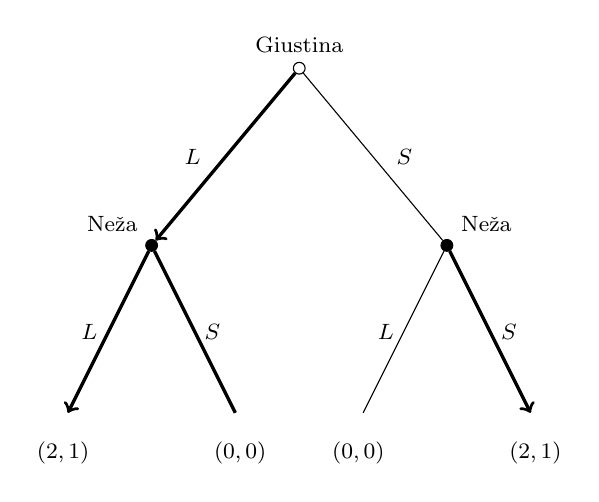
\begin{tikzpicture}[scale=1.5,font=\footnotesize, edge from parent/.style={draw}]
      \tikzstyle{solid node}=[circle,draw,inner sep=1.5,fill=black]
      \tikzstyle{hollow node}=[circle,draw,inner sep=1.5]
      \tikzstyle{level 1}=[level distance=15mm,sibling distance=2.5cm]
      \tikzstyle{level 2}=[level distance=15mm,sibling distance=1.5cm]
      \node(0)[hollow node,label=above:{Giustina}]{}
          child{node(1)[solid node,label=above left:{Ne\v{z}a}]{}
              child{node[label=below:{$(2,1)$}]{} edge from parent[->, very thick] node[left]{$L$}}
              child{node[label=below:{$(0,0)$}]{} edge from parent node[right]{$S$}}
              edge from parent[->, very thick] node[left,xshift=-5]{$L$}
          }
          child{node(2)[solid node,label=above right:{Ne\v{z}a}]{}
              child{node[label=below:{$(0,0)$}]{} edge from parent node[left]{$L$}}
              child{node[label=below:{$(2,1)$}]{} edge from parent[->, very thick] node[right]{$S$}}
              edge from parent node[right,xshift=5]{$S$}
          };
  \end{tikzpicture}\
  SPNE: 
  $\{(L)_G, (L\text{ if L}, S\text{ if S})_N\}$
  \task Normal form w/ underlined BR payoffs: \\
  \begin{tabular}{*{6}{c|}}
      \multicolumn{2}{c}{} & \multicolumn{4}{c}{Ne\v{z}a} \\ \cline{3-6}
      \multicolumn{1}{c}{} &  & $L,L$ & $L,S$ & $S,L$ & $S,S$ \\ \cline{2-6} 
      \multirow{2}*{Giustina}
      & $L$ & \underline{2}, \underline{1} &  \underline{2}, \underline{1} & 0, 0 & 0, 0 \\ \cline{2-6}
      & $S$ & 0, 0 &  1, \underline{2} & 0, 0 & \underline{1}, \underline{2} \\ \cline{2-6} 
  \end{tabular} \\
  $\{(L)_G, (L\text{ if L}, L\text{ if S})_N\}$
  is an NE but not SPNE
  because Ne\v{z}a would be irrational to pick Lion and Owl
  in the off-equilibrium path after Giustina goes to Spice N Steam. \\
  $\{(S)_G, (S\text{ if L}, S\text{ if S})_N\}$
  is another NE that is not sub-game perfect
  because Ne\v{z}a would be irrational to pick Spice N Steam
  in the off-equilibrium path after Giustina goes to Lion and Owl. \\
  \end{tasks}
\end{solution}
\end{question}

\newpage
%------------------------------------------------------------------

\begin{question}%[20]
Consider the strategic form game below:
\begin{table}[!h]
  \begin{center}
    \begin{tabular}{*{6}{c|}}
      \multicolumn{2}{c}{} & \multicolumn{4}{c}{$P_2$} \\ \cline{3-6}
      \multicolumn{1}{c}{} &  & $A$ & $B$ & $C$ & $D$ \\ \cline{2-6} 
      \multirow{4}*{$P_1$}
      & $W$ & 15, -7 &  8,  2 & 18, -7 & 11,  5 \\ \cline{2-6}
      & $X$ & -3, 18 &  6, -7 &  8, -7 & 17, 18 \\ \cline{2-6} 
      & $Y$ &  9, 19 & 20, -4 & 13,  6 & 10, 16 \\ \cline{2-6} 
      & $Z$ & -9, 20 & 14, 16 & 15, -5 & -3,  4 \\ \cline{2-6} 
  \end{tabular}
  \end{center}
\end{table}
\begin{tasks}
  \task 
  Use Iterated Deletion of Strictly Dominated Strategies
  and write out a simplified game table with any remaining cells.
  \task
  Find all Nash equilibria in \textit{pure strategies}.
  Explain why you know they are Nash equilibria.
  % \item 
  % Define mixed strategies for each player
  % using any pure strategies left after IDSDS.
  % Make sure to define all variables you introduce.
  % \item
  % Graph each player's expected utilities as functions of the 
  % other players' mixed strategy you defined in part (c).
  % \item
  % Solve for all Mixed Strategy Nash equilibria in this game.
  % A complete answer will include all calculations used 
  % and a graph of best response functions.
\end{tasks}
\begin{solution}
  \begin{tasks}
    \task
    \begin{enumerate}
      \item $C$ strictly dominated by $A$
      \item $Z$ is now SD by $Y$
      \item $B$ is now SD by $A$
      \item $Y$ is now SD by $W$
      \item no more SD strats, so stop IDSDS
    \end{enumerate}
      \begin{center}
        \begin{tabular}{*{4}{c|}}
          \multicolumn{2}{c}{} & \multicolumn{2}{c}{$P_2$} \\ \cline{3-4}
          \multicolumn{1}{c}{} &     & $A$    & $D$ \\ \cline{2-4}
          \multirow{2}*{$P_1$} & $W$ & \underline{15}, -7 & 11, \underline{5} \\ \cline{2-4}
                               & $X$ & -3, \underline{18} & \underline{17}, \underline{18} \\ \cline{2-4}
        \end{tabular}
      \end{center}
      \task
      NE: $\{X,D\}$ \\
      $X$ is BR to $D$, so $P_1$ has no regrets. \\
      $D$ is BR to $X$, so $P_2$ has no regrets. \\
      neither has any incentive to unilaterally deviate their own strategy.
  \end{tasks}
\end{solution}
\end{question}

\newpage

%------------------------------------------------------------------

\begin{question}
Consider the strategic form game below:
\begin{table}[h!]
  \begin{center}
  \begin{tabular}{*{5}{c|}}
    \multicolumn{2}{c}{} & \multicolumn{3}{c}{Aslanbek} \\\cline{3-5}
    \multicolumn{1}{c}{} & & $Low$ & $Moderate$ & $High$ \\\cline{2-5}
    \multirow{3}*{Hagano}  & $Low$ & 0,0 & 3,2 & 7,3 \\\cline{2-5}
                         & $Moderate$ & 2,3 & 5,5 & 6,4 \\\cline{2-5}
                         & $High$ & 3,7 & 4,6 & 4,5 \\ \cline{2-5}
  \end{tabular}
  \end{center}
\end{table}
\begin{tasks}
  \task
  Find all pure Nash strategy profiles when both play \textit{simultaneously}.
  \task
  Find all pure Nash strategy profiles when \textit{Hagano goes first}.
  Carefully explain all strategy profiles.
\end{tasks}
\begin{solution}
  \begin{tasks}
    \task There are three simultaneous pure strategy NE:
    $\{H_h,L_a\}$, $\{M_h, M_a\}$, and $\{L_h,H_a\}$
    \task 
    There is only one SPNE when Hagano goes first:
    \begin{itemize}
      \item Hagano plays $Low$
      \item Aslanbeck plays:
      \begin{itemize}
        \item $High$ if Hagano plays $High$
        \item $Moderate$ if Hagano plays $Moderate$
        \item $Low$ if Hagano plays $Low$
      \end{itemize}
    \end{itemize}
  \end{tasks}
\end{solution}
\end{question}

\newpage

%------------------------------------------------------------------

\begin{question}
Akua, Barta, and Gilberta are playing a version of hide and seek.
There are only two good hiding spots;
up a tree, or behind a rock.
Akua gets to hide first.
Barta also hides, but she gets to see which spot Akua is hiding
before she picks.
Once Akua and Barta are hidden,
Gilberta has to choose one and only one place to look.
If there are two people hiding in the same spot, 
they crowd each other and Gilberta can see them.
If there is only one person in a spot, Gilberta can't see 
who's hiding there. \\
Create an extensive form game tree
and clearly specify Gilberta's information set.
\begin{solution}
  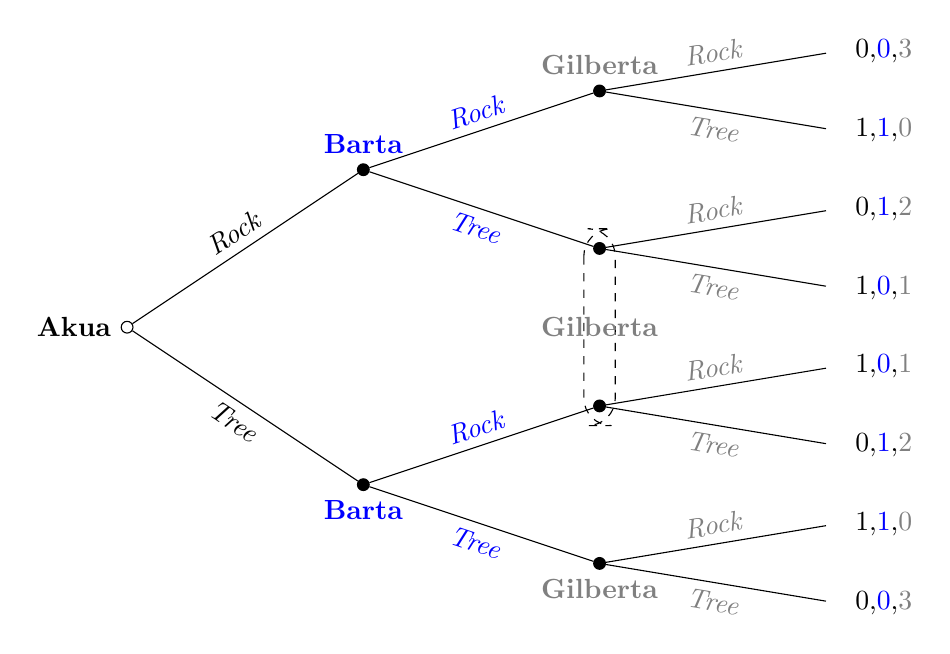
\begin{tikzpicture}[
  grow=right, 
  %edge from parent/.style={draw, very thick},
  level distance = 40mm,
  sibling distance = 25mm,
  %label distance = 1mm
  ]
  \tikzstyle{solid node}=[circle,draw,inner sep=1.5,fill=black]
  \tikzstyle{hollow node}=[circle,draw,inner sep=1.5]
  \tikzstyle{level 1}=[level distance=3cm,sibling distance=4cm]
  \tikzstyle{level 2}=[level distance=3cm,sibling distance=2cm]
  \tikzstyle{level 3}=[level distance=3cm,sibling distance=1cm]
 \node(0)[hollow node, label=left:{\textbf{Akua}}]{}
      child{node(1)[solid node, label=below:{\textbf{\color{blue} Barta}}]{}
          child{node()[solid node, label=below:{\textbf{\color{gray} Gilberta}}]{} 
              child{node[label=right:{0,{\color{blue}0},{\color{gray}3}}]{}
                  edge from parent node[below, sloped]{\textit{\color{gray} Tree}}
              }
              child{node[label=right:{1,{\color{blue}1},{\color{gray}0}}]{}
                  edge from parent node[above, sloped]{\textit{\color{gray} Rock}}
              }
              edge from parent node[below, sloped]{\textit{\color{blue} Tree}}
          }
          child{node(4)[solid node]{}
              child{node[label=right:{0,{\color{blue}1},{\color{gray}2}}]{}
                  edge from parent node[below, sloped]{\textit{\color{gray} Tree}}
              }
              child{node[label=right:{1,{\color{blue}0},{\color{gray}1}}]{}
                  edge from parent node[above, sloped]{\textit{\color{gray} Rock}}
              }
              edge from parent node[above, sloped]{\textit{\color{blue} Rock}}
          }
          edge from parent node[below, sloped]{\textit{Tree}}
      }
      child{node(2)[solid node, label=above:{\textbf{\color{blue} Barta}}]{}
          child{node(3)[solid node]{} 
              child{node[label=right:{1,{\color{blue}0},{\color{gray}1}}]{}
                  edge from parent node[below, sloped]{\textit{\color{gray} Tree}}
              }
              child{node[label=right:{0,{\color{blue}1},{\color{gray}2}}]{}
                  edge from parent node[above, sloped]{\textit{\color{gray} Rock}}
              }
              edge from parent node[below, sloped]{\textit{\color{blue} Tree}}
          }
          child{node()[solid node, label=above:{\textbf{\color{gray} Gilberta}}]{}
              child{node[label=right:{1,{\color{blue}1},{\color{gray}0}}]{}
                  edge from parent node[below, sloped]{\textit{\color{gray} Tree}}
              }
              child{node[label=right:{0,{\color{blue}0},{\color{gray}3}}]{}
                  edge from parent node[above, sloped]{\textit{\color{gray} Rock}}
              }
              edge from parent node[above, sloped]{\textit{\color{blue} Rock}}
          }
          edge from parent node[above, sloped]{\textit{Rock}}
      };
      \draw[dashed,rounded corners=10]($(3) + (-.2,.25)$)rectangle($(4) +(.2,-.25)$);
      \node at($(3)!.5!(4)$){\textbf{\color{gray} Gilberta}};
  \end{tikzpicture} \\
  \underline{Gilberta's information set:}
  \begin{itemize}
    \item Either both players are behind the Tree,
    \item or both players are behind the Rock,
    \item or: either Akua is behind the Rock and Bartua is behind the Tree;
    or Akua is behind the Tree and Bartua is behind the Rock
    (represented on the tree by the circled nodes)
  \end{itemize}
\end{solution}
\end{question}

\newpage

%------------------------------------------------------------------

\begin{question}
Suppose that two fishing boats are selling to the same market.
Let $V$ be the tons of fish caught by Vlatislav's boat,
and $J$ be the tons of fish caught by Jeren's boat.
People in this town only want to buy so many fish,
so the price $P$ of fish is given by the inverse demand function:
  $$P = 60 - (V+J)$$
Assume that Vlatislav has a marginal cost of 30
and Jeren has a marginal cost of 36.
\begin{tasks}
  \task Solve for Vlatislav's best response rule
  as a function of $J$.
  \task Solve for Jeren's best response rule
  as a function of $K$.
  \task
  Graph both players' best response functions 
  and find all Nash Equilibria.
  Label your graph appropriately.
\end{tasks}
\begin{solution}
  \begin{tasks}
    \task
    \begin{align*}
      \Pi_v & = (60 - V - J)V - 30 V \\
            & = 60V - V^2 - VJ - 30 V \\
      \frac{d\Pi_v}{dV} & = 60 - 2V - J - 30 \\
      BR_V(J) & = \frac{60-30-J}{2} = 15 - \frac{J}{2}
    \end{align*}
  \task
  \begin{align*}
      \Pi_j & = (60 - V - J)J - 36 J \\
      \frac{d\Pi_j}{dJ} & = 60 - 2J - V - 36 \\
      BR_V(J) & = \frac{60-36-V}{2} = 12 - \frac{V}{2}
  \end{align*}
  \task
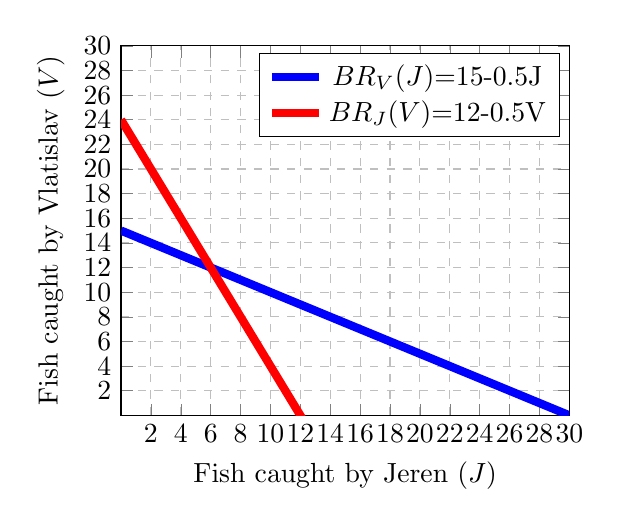
\begin{tikzpicture}
  \begin{axis}[
    width=0.6\textwidth,
    grid,
    ylabel={Fish caught by Vlatislav ($V$)},
    xlabel={Fish caught by Jeren ($J$)},
    xmin=0, xmax=30,
    ymin=0, ymax=30,
    xtick={2,4,...,30},
    ytick={2,4,...,30},
    grid style=dashed,
    ]
    \addplot [
        domain=0:30,
        line width=3pt,
        color=blue,
        ] 
        {15-0.5*x};
        \addlegendentry{\(BR_V(J)\)=15-0.5J}
        \addplot [
        domain=0:30,
        line width=3pt,
        color=red,
        ] 
        {24-2*x};
        \addlegendentry{\(BR_J(V)\)=12-0.5V}
    \addplot[draw=none] coordinates {(1,1)};
  \end{axis}
\end{tikzpicture} \\
\underline{NE:} $(J=6, J=12)$ is the only strategy profile
where both players' best responses intersect.
  \end{tasks}
\end{solution}
\end{question}
%------------------------------------------------------------------

\end{document}
